\documentclass[letterpaper,11pt,oneside,reqno]{article}

%%%%%%%%%%%%%%%%%%%%%%%%%%%%%%%%%%%%%%%%%%%%%%%%%%%%%%%%%%%%

\usepackage[pdftex,backref=page,colorlinks=true,linkcolor=blue,citecolor=red]{hyperref}
\usepackage[alphabetic, nobysame]{amsrefs}

%%%%%%%%%%%%%%%%%%%%%%%%%%%%%%%%%%%%%%%%%%%%%%%%%%%%%%%%%%%%
%main packages
\usepackage{amsmath,amssymb,amsthm,amsfonts,mathtools}
\usepackage{graphicx}
\usepackage[dvipsnames,svgnames]{xcolor}
\usepackage{upgreek}
\usepackage[mathscr]{euscript}

%equations
\allowdisplaybreaks
\numberwithin{equation}{section}

%tikz
\usepackage{tikz}
\usetikzlibrary{shapes,arrows,positioning,decorations.markings,decorations.pathreplacing}

%conveniences
\usepackage{array}
\usepackage{adjustbox}
\usepackage{cleveref}
\usepackage{enumerate}

%paper geometry
\usepackage[DIV=12]{typearea}
\usepackage{caption}
\captionsetup{width=.9\textwidth}

%%%%%%%%%%%%%%%%%%%%%%%%%%%%%%%%%%%%%%%%%%%%%%%%%%%%%%%%%%%%
%draft-specific
\synctex=1
% \usepackage{refcheck,comment}

%%%%%%%%%%%%%%%%%%%%%%%%%%%%%%%%%%%%%%%%%%%%%%%%%%%%%%%%%%%%
%this paper specific
\newcommand{\ssp}{\hspace{1pt}}

%%%%%%%%%%%%%%%%%%%%%%%%%%%%%%%%%%%%%%%%%%%%%%%%%%%%%%%%%%%%
\newtheorem{proposition}{Proposition}[section]
\newtheorem{lemma}[proposition]{Lemma}
\newtheorem{corollary}[proposition]{Corollary}
\newtheorem{theorem}[proposition]{Theorem}
\newtheorem{conjecture}[proposition]{Conjecture}
%%%%%%%%%%%%%%%%%%%%%%%%%%%%%%%%%%%%%%%%%%%%%%%%%%%%%%%%%%%%
\theoremstyle{definition}
\newtheorem{definition}[proposition]{Definition}
\newtheorem{remark}[proposition]{Remark}
%%%%%%%%%%%%%%%%%%%%%%%%%%%%%%%%%%%%%%%%%%%%%%%%%%%%%%%%%%%%
\Crefname{conjecture}{Conjecture}{Conjectures}

\begin{document}
\title{Colored interlacing triangles and Genocchi medians}

% OTHER AUTHORS

\author{Natasha Blitvic and Leonid Petrov}

\date{}

\maketitle

\begin{abstract}
Colored interlacing triangles, introduced by Aggarwal--Borodin--Wheeler (2024), provide the combinatorial framework for
the Central Limit Theorem for probability measures arising from the Lascoux--Leclerc--Thibon (LLT) polynomials.
Colored interlacing triangles depend on two key parameters: the number of colors $n$ and the depth of the triangle $N$. Recent work of Gaetz--Gao (2025) connects these objects to Schubert calculus and resolves the enumeration for $n=3$ and arbitrary depth $N$. However, the enumerative behavior for general $n$ has remained open.

In this paper, we analyze the complementary regime: fixed depth $N=2$ and arbitrary number of colors $n$. We prove that in this setting, colored interlacing triangles are in bijection with Dumont derangements, identifying their enumeration with the Genocchi medians. This connects the probabilistic model to a rich hierarchy of classical combinatorial objects.

Furthermore, we introduce a $q$-deformation of this enumeration arising naturally from the LLT transition energy. This yields new $q$-analogs of the Genocchi medians.
Finally, we present computational results
and sampling algorithms
for colored interlacing triangles with higher $N$ or $n$, which
suggests the limits of combinatorial tractability in the $(N,n)$ parameter space.
\end{abstract}

\section{Introduction}
\label{sec:intro}

\subsection{Overview}

Colored interlacing triangles were introduced by Aggarwal--Borodin--Wheeler \cite{ABW2023coloured_LLT}
as discrete objects arising in the study of Gaussian limits of probability measures
coming from Cauchy identities for LLT (Lascoux--Leclerc--Thibon) polynomials.
The pre-limit \emph{LLT processes}
live on tuples of semistandard Young tableaux, and 
generalize Schur processes
of Okounkov--Reshetikhin
\cite{okounkov2003correlation}.
The Central Limit Theorem behavior of the latter 
is described by the joint law of eigenvalues of corners of random matrices from the
Gaussian Unitary Ensemble (GUE),
see Okounkov--Reshetikhin \cite{OkounkovReshetikhin2006RandomMatr} and 
Gorin--Panova \cite{GorinPanova2012_full}.
In the LLT generalization (which also contains a deformation
parameter $q$), along with the continuous GUE corners components,
one also obtains a $q$-measure on the space of certain discrete 
objects, the \emph{colored interlacing triangles}.

In this paper, we study combinatorial aspects of colored interlacing triangles
in their own right, focusing on enumeration, bijections, $q$-counting, and
random sampling. In particular, we obtain an exact enumeration of depth-$2$
triangles in terms of Genocchi medians, explore a $q$-deformation of the general
enumeration problem, and provide computational results for higher depths,
including a disproof of \cite[Conjecture~A.5]{ABW2023coloured_LLT}.

\subsection{Colored interlacing triangles}

\begin{definition}
	\label{def:colored_interlacing_triangle}
	Fix $n,N\ge1$. We call $N$ the \emph{depth} of a triangle, and $n$ is the \emph{number of colors}.
	A (\emph{colored}) \emph{interlacing $n$-triangle} 
	$\boldsymbol\lambda$
	is a collection of
	$nN(N+1)/2$ colored dots (represented by numbers),
	arranged into $n$ triangles of depth $N$,
	with
	each triangle consisting of
	$1$ dot at the bottommost level, $2$ dots at the next level, and so on, up to $N$ dots at the top level.
	We denote
	by $\lambda[i]^{k}_{j}
	\in\left\{ 1,\ldots,n  \right\}$
	the color
	of the
	dot which is located in the $i$-th triangle, on the $k$-th level, and at the $j$-th position from the left.
	For any level
	$k=1,\ldots,N-1$,
	define a \emph{linear order}
	between dots at levels $k$ and $k+1$ as follows:
	\begin{equation}
		\label{eq:interlacing_order}
		\lambda[1]^{k+1}_{1}
		\Big\vert
		\lambda[1]^{k}_{1}
		\Big\vert
		\lambda[1]^{k+1}_{2}
		\ldots
		\lambda[1]^{k+1}_{k}
		\Big\vert
		\lambda[1]^k_k
		\Big\vert
		\lambda[1]^{k+1}_{k+1}
		\lambda[2]^{k+1}_1
		\Big\vert
		\lambda[2]^k_1
		\ldots
		\lambda[n]^{k+1}_k
		\Big\vert
		\lambda[n]^k_k
		\Big\vert
		\lambda[n]^{k+1}_{k+1},
	\end{equation}
	where the vertical bars separate the entries from different levels.
	Denote by
	$\lambda^{k}=(\lambda^k_1,\lambda^k_2,\ldots,\lambda^k_{nk})$ the sequence of elements in the $k$-th row, read from left to right
	according to the linear order \eqref{eq:interlacing_order}.
	This notation suppresses the triangle index $[i]$, treating the entire level as a single row of length $nk$,
	which is especially helpful when dealing with small-$N$ cases.
	
	By definition, the interlacing $n$-triangle must satisfy two conditions:
	\begin{enumerate}[$\bullet$]
		\item For each color $b\in\left\{ 1,\ldots,n \right\}$
			and any level number $k=1,\ldots,N$,
			there are exactly $k$ dots of color $b$ on the $k$-th level in the union of all triangles.
		\item
			For each color $b\in\left\{ 1,\ldots,n \right\}$
			and any level $k=1,\ldots,N-1$, the configurations
			of color-$b$ dots at levels $k$ and $k+1$ must \emph{interlace} (notation $\lambda^k\prec \lambda^{k+1}$).
			That is,
			between any two dots of color $b$ at level $k+1$, there is exactly one dot of color $b$ at level $k$.
			Here ``between'' is understood
			in the sense of the linear order \eqref{eq:interlacing_order}.
	\end{enumerate}
	See \Cref{fig:small_interlacing_example} for an example. In particular, for this $\boldsymbol\lambda$ we
	have $\lambda^1=(2,3,1)$, 
	$\lambda^2=(2,1,3,3,2,1)$,
	and 
	$\lambda^3=(2,1,2,3,3,1,3,2,1)$.

	We denote the set of all colored interlacing $n$-triangles
	of depth $N$,
	\begin{equation}
		\label{eq:bold_lambda_notation}
		\boldsymbol\lambda=\bigl\{\lambda[i]^{k}_{j}\colon 1\le i\le n,\ 1\le j\le k\le N\bigr\},
	\end{equation}
	$\mathcal{T}_N(n)$.
	Let $T_N(n)\coloneqq\#\mathcal{T}_N(n)$ be the number of such triangles.
\end{definition}
For future reference, let us denote by 
$\mathring{\mathcal{T}}_N(n)$ the subset of
$\mathcal{T}_N(n)$ consisting of triangles
with the identity permutation of colors at the bottom row, $\lambda^1 = (1,2,\ldots,n)$.
Clearly, simultaneous permutations of all $n$ colors do not affect the interlacing condition,
so we have
\begin{equation}
	\label{eq:fixed_bottom_row}
	T_N(n) = n! \cdot \# \mathring{\mathcal{T}}_N(n).
\end{equation}


\begin{figure}[htpb]
	\centering
	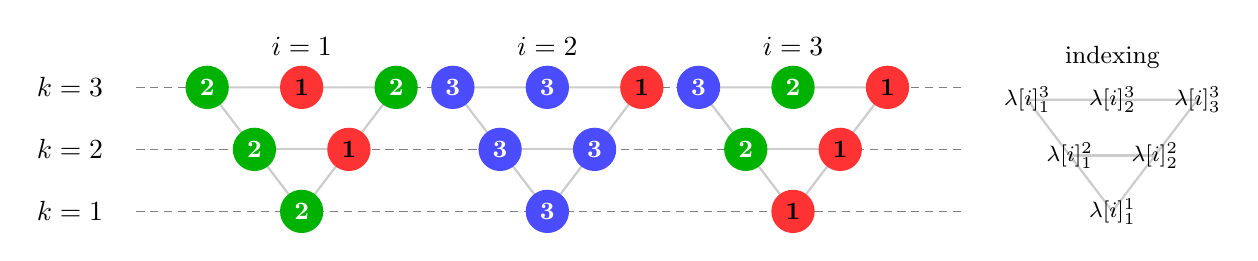
\begin{tikzpicture}
		[scale=0.75,
		 dot1/.style={circle, fill=red!80, minimum size=5.5mm, inner sep=0pt, font=\small\bfseries},
		 dot2/.style={circle, fill=green!70!black, minimum size=5.5mm, inner sep=0pt, font=\small\bfseries, text=white},
		 dot3/.style={circle, fill=blue!70, minimum size=5.5mm, inner sep=0pt, font=\small\bfseries, text=white}]
		\def\h{0.8}
		\def\v{1.05}
		\def\tsep{5.2*\h}
		% Level labels
		\node[left] at (-4*\h, 0) {$k=1$};
		\node[left] at (-4*\h, \v) {$k=2$};
		\node[left] at (-4*\h, 2*\v) {$k=3$};
		% Dashed level lines
		\draw[gray, densely dashed] (-3.5*\h,0) -- (14*\h,0);
		\draw[gray, densely dashed] (-3.5*\h,\v) -- (14*\h,\v);
		\draw[gray, densely dashed] (-3.5*\h,2*\v) -- (14*\h,2*\v);
		% Triangle 1: top (2,1,2), mid (2,1), bot (2)
		\begin{scope}[shift={(0,0)}]
			\draw[gray!40, thick] (-2*\h,2*\v) -- (2*\h,2*\v) -- (0,0) -- cycle;
			\draw[gray!40, thick] (-\h,\v) -- (\h,\v);
			\node[dot2] at (-2*\h,2*\v) {2};
			\node[dot1] at (0,2*\v) {1};
			\node[dot2] at (2*\h,2*\v) {2};
			\node[dot2] at (-\h,\v) {2};
			\node[dot1] at (\h,\v) {1};
			\node[dot2] at (0,0) {2};
			\node at (0,2*\v+0.7) {$i=1$};
		\end{scope}
		% Triangle 2: top (3,3,1), mid (3,3), bot (3)
		\begin{scope}[shift={(\tsep,0)}]
			\draw[gray!40, thick] (-2*\h,2*\v) -- (2*\h,2*\v) -- (0,0) -- cycle;
			\draw[gray!40, thick] (-\h,\v) -- (\h,\v);
			\node[dot3] at (-2*\h,2*\v) {3};
			\node[dot3] at (0,2*\v) {3};
			\node[dot1] at (2*\h,2*\v) {1};
			\node[dot3] at (-\h,\v) {3};
			\node[dot3] at (\h,\v) {3};
			\node[dot3] at (0,0) {3};
			\node at (0,2*\v+0.7) {$i=2$};
		\end{scope}
		% Triangle 3: top (3,2,1), mid (2,1), bot (1)
		\begin{scope}[shift={(2*\tsep,0)}]
			\draw[gray!40, thick] (-2*\h,2*\v) -- (2*\h,2*\v) -- (0,0) -- cycle;
			\draw[gray!40, thick] (-\h,\v) -- (\h,\v);
			\node[dot3] at (-2*\h,2*\v) {3};
			\node[dot2] at (0,2*\v) {2};
			\node[dot1] at (2*\h,2*\v) {1};
			\node[dot2] at (-\h,\v) {2};
			\node[dot1] at (\h,\v) {1};
			\node[dot1] at (0,0) {1};
			\node at (0,2*\v+0.7) {$i=3$};
		\end{scope}
		% Indexing notation (separate panel to the right)
		\begin{scope}[shift={(3.3*\tsep,0)}, scale=0.9]
			\draw[gray!40, thick] (-2*\h,2*\v) -- (2*\h,2*\v) -- (0,0) -- cycle;
			\draw[gray!40, thick] (-\h,\v) -- (\h,\v);
			\node[font=\footnotesize] at (-2*\h,2*\v) {$\lambda[i]^3_1$};
			\node[font=\footnotesize] at (0,2*\v) {$\lambda[i]^3_2$};
			\node[font=\footnotesize] at (2*\h,2*\v) {$\lambda[i]^3_3$};
			\node[font=\footnotesize] at (-\h,\v) {$\lambda[i]^2_1$};
			\node[font=\footnotesize] at (\h,\v) {$\lambda[i]^2_2$};
			\node[font=\footnotesize] at (0,0) {$\lambda[i]^1_1$};
			\node at (0,2*\v+0.8) {\small indexing};
		\end{scope}
	\end{tikzpicture}
	\caption{Left: A colored interlacing triangle with $n=3$ colors and $N=3$ levels.
	Colors: \textcolor{red!80}{1 (red)}, \textcolor{green!70!black}{2 (green)}, \textcolor{blue!70}{3 (blue)}.
	Right: indexing notation $\lambda[i]^k_j$ for the $i$-th triangle.
	Row sequences:
	$\lambda^{1}=(\textcolor{green!70!black}{2},\textcolor{blue!70}{3},\textcolor{red!80}{1})$,
	$\lambda^{2}=(\textcolor{green!70!black}{2},\textcolor{red!80}{1},\textcolor{blue!70}{3},\textcolor{blue!70}{3},\textcolor{green!70!black}{2},\textcolor{red!80}{1})$,
	$\lambda^{3}=(\textcolor{green!70!black}{2},\textcolor{red!80}{1},\textcolor{green!70!black}{2},\textcolor{blue!70}{3},\textcolor{blue!70}{3},\textcolor{red!80}{1},\textcolor{blue!70}{3},\textcolor{green!70!black}{2},\textcolor{red!80}{1})$. Each pair of consecutive rows 
	may be written in one line using the linear order \eqref{eq:interlacing_order}, for 
	example,
	$(2|2|13|3|32|1|1)$ for the first two levels.}
	\label{fig:small_interlacing_example}
\end{figure}

Let us briefly mention the probabilistic origin of these objects
from Aggarwal--Borodin--Wheeler \cite{ABW2023coloured_LLT}.
The LLT (Lascoux--Leclerc--Thibon) polynomials \cite{lascoux1997ribbon}
are a rank-$n$, $q$-deformation of products of Schur polynomials,
reducing to the latter when $q=1$.
Throughout the paper, we refer to $n$ as the \emph{number of colors}.
Similarly to the Schur case \cite{fulman1997probabilistic},
\cite{okounkov2001infinite},
\cite{okounkov2003correlation}, one can define probability measures
by normalizing Cauchy summation identities.
Among the measures one can obtain in this manner are
coupled tuples of domino tilings of the Aztec diamond 
introduced by Corteel--Gitlin--Keating \cite{corteel2023ktilings},
see also \cite{keating2024shuffling} for a sampling algorithm generalizing
classical domino shuffling to the coupled setting.

Aggarwal--Borodin--Wheeler \cite{ABW2023coloured_LLT}
studied Central Limit Theorems for measures based on LLT polynomials.
In the Schur case, the role of the Gaussian distribution in this 
regime is played by the corners process of the 
Gaussian Unitary Ensemble (GUE) of random matrix theory
\cite{OkounkovReshetikhin2006RandomMatr}, \cite{GorinPanova2012_full}.
That is, one considers the joint distribution of eigenvalues of all top-left corners
of a random Gaussian Hermitian matrix, and this joint distribution describes
the limiting fluctuations of Schur processes.

Generalizing to the LLT level, one obtains a more complex limit object.
Namely, the distribution describing the fluctuations of LLT processes
splits into two independent parts:
a \emph{continuous part}, which is a product of $n$ independent
GUE (Gaussian Unitary Ensemble) corners processes,
and a \emph{discrete part}, which is a $q$-weighted probability distribution
on the finite set $\mathcal{T}_N(n)$ of colored interlacing triangles 
from \Cref{def:colored_interlacing_triangle}.
The discrete part is nontrivial for $n>1$, while for 
$n=1$ (Schur case), one has a single copy of the GUE corners process.

The combinatorial landscape of colored interlacing triangles is vast,
parameterized by the number of colors $n$ and the depth $N$. A complete
understanding requires exploring both dimensions.
Aggarwal--Borodin--Wheeler \cite{ABW2023coloured_LLT} initiated the study of enumeration
for fixed $n$, observing that $T_N(2) = 2^N$ since two-colored interlacing triangles
are isomorphic to binary trees \cite[Proposition~A.1]{ABW2023coloured_LLT}.
They conjectured \cite[Conjecture~A.3]{ABW2023coloured_LLT} that
$T_N(3) = \frac{1}{4}\mathfrak{g}_N^{\Delta}(4)$,
where $\mathfrak{g}_N^{\Delta}(4)$ \cite[A153467]{OEIS}
is the number of $4$-colorings of a triangular grid of side length $N$.
This was proved by Gaetz and Gao \cite{gaetz2023bijection}, who uncovered
deep connections to Schubert calculus.
We independently observed that \cite[Conjecture~A.5]{ABW2023coloured_LLT}, which posited
$T_N(4) = \frac{1}{5}\mathfrak{g}_N^{*}(5)$
(where $\mathfrak{g}_N^{*}(5)$ \cite[A068294]{OEIS} counts $5$-colorings of an octagonal array),
fails for $N \ge 3$; this was also reported by \cite{gaetz2023bijection}.

The present work complements these fixed-$n$ results by exploring the ``horizontal'' direction
($N=2$, arbitrary $n$). By fixing the depth, we let the number of
colors grow indefinitely, revealing a connection to the classical Genocchi
numbers that is invisible when $n$ is fixed.
This result, together with
\cite{gaetz2023bijection}, maps out the landscape 
of so far available enumerative results for colored interlacing triangles:
the vertical direction
connects to geometry, while the horizontal direction
connects to the classical theory of permutation statistics, and presentrs
a straightforward path to interpreting $q$-analogs coming from the
Central Limit Theorem for measures based on LLT polynomials.

In the next \Cref{subsec:main_results}, we summarize our main results
on enumeration and $q$-counting in the discrete space $\mathcal{T}_N(n)$.

\subsection{Main results and outline of the paper}
\label{subsec:main_results}

Our primary contribution is the complete resolution of the enumeration problem for the $N=2$ slice of the hierarchy. In \Cref{sec:genocchi_case}, we prove that depth-$2$ colored interlacing triangles are in bijection with Dumont derangements, identifying their partition function with the Genocchi medians $H_n$ and connecting the probabilistic model to classical combinatorial objects. Building on this, in \Cref{sec:q_enumeration}, we analyze the intrinsic LLT $q$-statistic defined in \cite{ABW2023coloured_LLT}; we show that for $N=2$, this ``energy'' of inter-level transitions leads to $q$-analogs of the Genocchi medians distinct from all previously known $q$-analogs.

Probing the hierarchy beyond $N=2$, in \Cref{subsec:computational_approach} we enumerate $\mathcal{T}_N(n)$ for a range of depths and sizes, finding that the counts exhibit large prime factors and eventually hit computational walls --- evidence that the combinatorics diverges from the closed-form patterns of the Genocchi case or the Schubert calculus connections at $n=3$.
Along the way, we provide independent confirmation of the disproof of \cite[Conjecture~A.5]{ABW2023coloured_LLT}. 

Returning to depth $N=2$, in \Cref{subsec:q_data,subsec:conjectures_on_coefficients,subsec:linear_cumulant_phenomenon} we perform a detailed
computational
study of the $q$-Genocchi medians. We derive conjectured formulas for coefficients of low powers of $q$ (which we prove for the first power, see \Cref{prop:linear_coefficient}), and observe a curious ``linear cumulant'' phenomenon in the distribution of the $q$-statistic. 

Finally, in \Cref{sec:sampling}, we develop a Markov Chain Monte Carlo algorithm for sampling from the $q$-weighted measure on $\mathcal{T}_2(n)$.

\subsection{Acknowledgments}

LP was partially supported by the NSF grant DMS-2153869 and by the
Simons Foundation Travel Support for Mathematicians Awards.
Part of this research was performed in Spring 2024
while LP was
visiting the
program
``Geometry, Statistical Mechanics, and Integrability''
at the Institute for Pure and Applied Mathematics
(IPAM), which is supported by the NSF grant DMS-1925919. NB was partially supported by the EPSRC grant EP/V048902. We thank Amol Aggarwal and Alexei Borodin for helpful discussions.

%%%%%%%%%%%%%%%%%%%%%%%%%%%%%%%%%%%%%%%%%%%%%%%%%%%%%%%%%%%%%%%%%%%%%%%%%%%%%%%
\section{Two-level colored interlacing triangles and Genocchi medians}
\label{sec:genocchi_case}
%%%%%%%%%%%%%%%%%%%%%%%%%%%%%%%%%%%%%%%%%%%%%%%%%%%%%%%%%%%%%%%%%%%%%%%%%%%%%%%

In this section, we establish the enumeration formula for depth-$2$ colored interlacing triangles
in terms of Genocchi medians.

The sequence of Genocchi medians $H_n$ (also sometimes called the Genocchi numbers of 
second kind) is a 
classical integer sequence in combinatorics with several interpretations.
We refer to \cite{Dumont1974}, \cite{DumontRandrianarivony1994}, and 
the entry \cite[A005439]{OEIS} for background and further references.
The following definition in terms of a certain class of permutations
(called the \emph{Dumont derangements}) goes back to
\cite{Dumont1974}:

\begin{definition}
	\label{def:derrangement}
	A permutation $\sigma\in S_{2n}$ is called
	a \emph{Dumont derangement} (of second kind)
	if the following two conditions hold:
	\begin{equation*}
		\begin{cases}
			i< \sigma(i),& \textnormal{for all $i$ odd};
			\\
			i> \sigma(i),& \textnormal{for all $i$ even}.
		\end{cases}
	\end{equation*}
	The number of Dumont derangements in $S_{2n}$
	is called the $n$-th \emph{Genocchi median} and denoted by~$H_n$.
	We have
	\begin{equation*}
		H_0=H_1=1,\quad
		H_2=2,\quad
		H_3=8,\quad
		H_4=56,\quad
		H_5=608,\quad
		\ldots
	\end{equation*}
\end{definition}

Recall that we denote by $T_N(n)$ the number of colored interlacing $n$-triangles of depth $N$
(\Cref{def:colored_interlacing_triangle}).
\begin{theorem}
	\label{thm:Genocchi_counts}
	We have
	$T_2(n)=n!\cdot H_n$ for all $n\geq 0$.
\end{theorem}
\begin{proof}
It suffices to show that $\# \mathring{\mathcal{T}}_2(n) = H_n$, see 
\eqref{eq:fixed_bottom_row}.
Let us identify 
the valid top rows 
with Dumont derangements in~$S_{2n}$.

The top row is a sequence of $2n$ elements where each color appears exactly twice.
For a color~$c=1,\ldots,n $, let $p_1 < p_2$ be the positions of its two occurrences,
and define $\sigma \in S_{2n}$ by
\begin{equation*}
\sigma(2c) = p_1, \qquad \sigma(2c-1) = p_2.
\end{equation*}
The interlacing condition requires that the color $c$ at level $1$ 
lies strictly between the two level-$2$ positions of $c$.
This means that $p_1 < 2c$ and $p_2 > 2c-1$,
which are precisely the Dumont derangement conditions.
This completes the bijective proof.
\end{proof}

The interpretation in terms of colored interlacing triangles yields the following
well-known divisibility property of the Genocchi medians:
\begin{corollary}
\label{cor:Genocchi_divisibility}
	The number $H_n$ is divisible by $2^{n-1}$.
\end{corollary}
\begin{proof}
	Consider the set $\mathring{\mathcal{T}}_2(n)$.
	For each $i=1,\ldots,n-1 $, 
	the entries $\lambda[i]^2_2$ and $\lambda[i+1]^2_1$
	are immediate neighbors in the linear order \eqref{eq:interlacing_order},
	with no entries between them at level $1$. 
	Therefore, $\lambda[i]^2_2 \ne \lambda[i+1]^2_1$.
	Swapping these two entries produces a different valid top row,
	and this operation can be performed independently for each $i$.
	This leads to $n-1$ independent involutions on $\mathring{\mathcal{T}}_2(n)$,
	which implies the divisibility.
\end{proof}

In the same manner, this divisibility property is generalized to an arbitrary depth:
\begin{proposition}
	\label{prop:divisibility_general_depth}
	For $N\ge2$, the number $T_N(n)/n!$ is divisible by $2^{n-1}$.
\end{proposition}
\begin{proof}
	There are $n-1$ independent involutions on $\mathring{\mathcal{T}}_N(n)$
	swapping the neighbors $\lambda[i]^N_N\ne \lambda[i+1]^N_1$ 
	at the top level.
\end{proof}

\begin{remark}
	\label{rem:divisibility_no_improvement}
	One might hope to improve the divisibility in \Cref{prop:divisibility_general_depth}
	to $2^{(n-1)(N-1)}$ by constructing 
	independent involutions at each of the $N-1$ levels $2\le k \le N$.
	However, as the hypothetical involutions at lower levels
	are constrained by the interlacing conditions imposed from above,
	this may not be possible. Indeed,
	exact enumeration 
	shows that such an improvement is not possible in general:
	$T_3(3)/3! = 88$ is divisible by $2^3$ but not by $2^{(3-1)(3-1)} = 16$
	(see \Cref{sec:enumeration} and \Cref{tab:2_adic_valuations} in particular).
\end{remark}

%%%%%%%%%%%%%%%%%%%%%%%%%%%%%%%%%%%%%%%%%%%%%%%%%%%%%%%%%%%%%%%%%%%%%%%%%%%%%%%
\section{The $q$-enumeration of colored interlacing triangles}
\label{sec:q_enumeration}
%%%%%%%%%%%%%%%%%%%%%%%%%%%%%%%%%%%%%%%%%%%%%%%%%%%%%%%%%%%%%%%%%%%%%%%%%%%%%%%

In this section, we explore the $q$-counting statistic
(we denote it by $\psi(\lambda^{k-1},\lambda^k)$)
on colored interlacing
triangles based on interactions between consecutive levels.
This statistic is related to the quantity $\xi(\cdot;\cdot)$
arising from the 
Central Limit Theorem for LLT processes
\cite[Section~1.6]{ABW2023coloured_LLT}.

For depth $N=2$, 
we obtain new $q$-analogs of the quantities $T_2(n)=n!\cdot H_n$,
distinct from previously known $q$-analogs of the Genocchi medians $H_n$.
We begin with a brief survey of three known $q$-analogs of the Genocchi medians.

\subsection{Known $q$-analogs of Genocchi medians}
\label{subsec:known_q_analogs}

Several $q$-analogs of the Genocchi medians can be obtained by $q$-deforming
the various classical definitions of these numbers, including
generating functions, recurrences, and combinatorial models obtained by assigning a
$q$-weight to the relevant objects (in particular, Dumont derangements).

First, Randrianarivony \cite{Randrianarivony1997}
simply weights each Dumont derangement $\sigma\in S_{2n}$ by the usual inversion number $\mathrm{inv}(\sigma)$,
and also provides
Stieltjes-type continued fraction expansions for the corresponding generating function.
The first few $q$-deformations from \cite{Randrianarivony1997} are:
\begin{equation}
\label{eq:Randrianarivony_q_Gandhi}
\begin{split}
H_1^R(q) &= q, \\
H_2^R(q) &= q^2 (1 + q), \\
H_3^R(q) &= q^3 (1 + q)^3 (1 - q + q^2), \\
H_4^R(q) &= q^4 (1 + q)^3 (1 + 2q^3 + q^5 + 2q^6 + q^7), \\
H_5^R(q) &= q^5 (1 + q)^5 (1 - q + q^2)^2 (1 + q + q^3 + q^4 + 2q^5 + 4q^6 + 5q^7 + 3q^8 + q^9).
\end{split}
\end{equation}

\medskip 
Second, 
Han and Zeng 
\cite{HanZeng1999Discrete},
\cite{HanZeng1999}
introduced polynomials $C_n(x,q)$
via a $q$-deformation of the classical Gandhi recurrence:
\begin{equation*}
\Delta_q f(x) = \frac{f(1+qx)-f(x)}{1+(q-1)x}, \quad C_1(x,q)=1, \quad C_n(x,q)
= (1+qx) \Delta_q \left( x C_{n-1}(x,q) \right), \quad n \ge 2.
\end{equation*}
The values at $x=1$ yield the following $q$-analogs of the Genocchi medians:
\begin{equation}
\label{eq:HanZeng_q_Gandhi}
\begin{split}
H_1^{HZ}(q) &= 1, \\ H_2^{HZ}(q) &= 1 + q, \\ H_3^{HZ}(q) &= (1+q)^3, \\
H_4^{HZ}(q) &= (1+q)^3 (1 + 3q + 2q^2 + q^3), \\
H_5^{HZ}(q) &= (1+q)^5 (1 + 5q + 5q^2 + 5q^3 + 2q^4 + q^5).
\end{split}
\end{equation}
These polynomials have a combinatorial interpretation in 
terms of a certain \emph{Denert statistic} on Dumont derangements
\cite{HanZeng1999Discrete},
which separately treats inversions between odd and even positions.
Feigin \cite{Feigin2012}
identified the polynomials
\eqref{eq:HanZeng_q_Gandhi} (divided by $(1+q)^{n-1}$)
as the Poincar\'e polynomials of degenerate flag varieties.

\medskip
Finally, the third $q$-analog was introduced by
Zeng and Zhou \cite{ZengZhou2006}
via a $q$-deformation of the Seidel
triangle recurrence
\cite{Seidel1877}:
\begin{align*}
g_{1,1}(q) &= g_{2,1}(q)=1,\\
g_{2i+1,j}(q) &= g_{2i+1,j-1}(q)+q^{j-1}g_{2i,j}(q), \\
g_{2i,j}(q) &= g_{2i,j+1}(q)+q^{j-1} g_{2i-1,j}(q).
\end{align*}
The $q$-Genocchi medians are $H_n^{ZZ}(q) := g_{2n,1}(q)$:
\begin{equation}
\label{eq:ZengZhou_q_Genocchi}
\begin{split}
H_1^{ZZ}(q) &= 1, \\ H_2^{ZZ}(q) &= 1 + q, \\ H_3^{ZZ}(q) &= (1 + q)^2 (1 + q^2), \\
H_4^{ZZ}(q) &= (1 + q)^2 (1 + q^2) (1 + q + q^2 + 2q^3 + q^4 + q^5), \\
H_5^{ZZ}(q) &= (1 + q)^3 (1 + q^2)^2 (1 - q + q^2) (1 + 2q + 2q^2 + 3q^3 + 4q^4 + 4q^5 + 2q^6 + q^7).
\end{split}
\end{equation}
These can also be interpreted in terms of a charge statistic on so-called strict alternating pistols~\cite{ZengZhou2006}.

\medskip

We see that all of these $q$-analogs
\eqref{eq:Randrianarivony_q_Gandhi},
\eqref{eq:HanZeng_q_Gandhi},
and
\eqref{eq:ZengZhou_q_Genocchi}
are different. Moreover, the divisibility by a power of $2$ in the original Genocchi medians
(\Cref{cor:Genocchi_divisibility}) 
is replaced by divisibility by a power of $(1+q)$.

\subsection{Inter-level statistic $\psi$ on colored interlacing triangles}
\label{subsec:inter_level_statistic}

The probability measure on colored interlacing triangles
coming from the Central Limit Theorem for LLT processes
\cite{ABW2023coloured_LLT}
is decomposed into a 
product of the top-row contribution
(involving a complicated vertex model with signed configuration weights, which we do not pursue 
here\footnote{However, for depth $N=1$, this complicated vertex model 
for the top row, denoted by $g_{\Delta}^{c^{[N]}}$ in \cite{ABW2023coloured_LLT},
yields the well-known Mallows measure on $S_n$,
under which a permutation $\sigma$ is weighted proportionally to $q^{\mathrm{inv}(\sigma)}$.})
and simpler inter-level contributions given by powers of $q$.
We focus on the latter: for each pair of consecutive levels
in a colored triangle, define a statistic $\psi(\lambda^{k-1}, \lambda^k)$, $k=2,\ldots,N$:

\begin{definition}[\cite{ABW2023coloured_LLT}]
	\label{def:psi}
	Fix $k=2,\ldots,N$, and let $\lambda^k=\nu$ and $\lambda^{k-1}=\mu$ 
	be two consecutive rows of a colored interlacing $n$-triangle $\boldsymbol\lambda$.
	Consider a one-row vertex model in which arrows can have 
	one of $n$ colors,
	the horizontal line can carry an arbitrary composition of colors,
	and vertical lines can carry only one color:
	\begin{equation}
		\label{eq:psi_factor_vertex_model}
		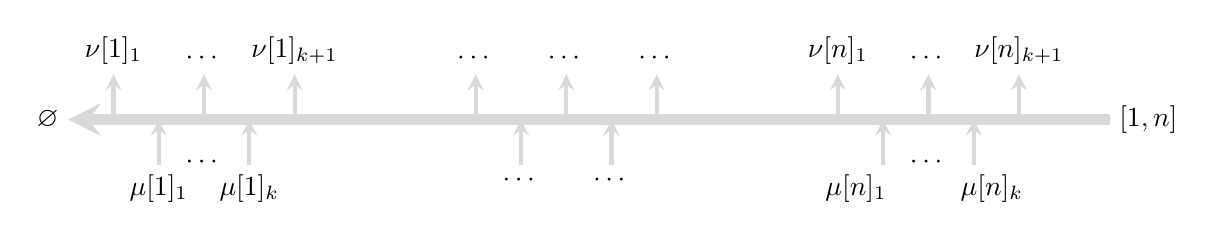
\begin{tikzpicture}
			[scale=1.15,baseline=(current bounding box.center),>=stealth]
			\colorlet{lgray}{white!85!black}
		\draw[lgray,line width=4pt,<-] (0.5,0) -- (12,0);
		\foreach\x in {1,2,3,5,6,7,9,10,11}{
		\draw[lgray,line width=1.5pt,->] (\x,0) -- (\x,0.5);
		}
		\node[above] at (1,0.5) {$\nu[1]_1$};
		\node[above] at (2,0.5) {$\cdots$};
		\node[above] at (3,0.5) {$\nu[1]_{k+1}$};
		%
		\node[above] at (5,0.5) {$\cdots$};
		\node[above] at (6,0.5) {$\cdots$};
		\node[above] at (7,0.5) {$\cdots$};
		%
		\node[above] at (9,0.5) {$\nu[n]_1$};
		\node[above] at (10,0.5) {$\cdots$};
		\node[above] at (11,0.5) {$\nu[n]_{k+1}$};
		%
		\foreach\x in {1.5,2.5,5.5,6.5,9.5,10.5}{
		\draw[lgray,line width=1.5pt,->] (\x,-0.5) -- (\x,0);
		}
		%
		\node[below] at (1.5,-0.5) {$\mu[1]_1$};
		\node[below] at (2,-0.3) {$\cdots$};
		\node[below] at (2.5,-0.5) {$\mu[1]_k$};
		%
		\node[below] at (5.5,-0.5) {$\cdots$};
		\node[below] at (6.5,-0.5) {$\cdots$};
		%
		\node[below] at (9.2,-0.5) {$\mu[n]_1$};
		\node[below] at (10,-0.3) {$\cdots$};
		\node[below] at (10.7,-0.5) {$\mu[n]_{k}$};
		%
		\node[left] at (0.5,0) {$\varnothing$}; \node[right] at (12,0) {$[1,n]$};
		\end{tikzpicture}
	\end{equation}
	Here, the incoming configuration from the right has an 
	arrow of each color $b=1,\ldots,n$,
	the outgoing configuration on the left is empty,
	and the colors are conserved in the direction of arrow flow.
	That is, there are two possible types of vertices:
	\begin{equation}
		\label{eq:psi_factor_two_types_of_vertices}
		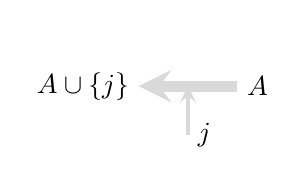
\begin{tikzpicture}
			[scale=1.25,baseline=(current bounding box.center),>=stealth]
				\colorlet{lgray}{white!85!black}
				\draw[lgray,line width=4pt,<-] (0.5,0) -- (1.5,0);
				\draw[lgray,line width=1.5pt,->] (1,-0.5) -- (1,0);
				\node[right] at (1,-0.5) {$j$};
				\node[left] at (0.5,0) {$A\cup \left\{ j \right\}$};
				\node[right] at (1.5,0) {$A$};
				\node at (1,0.5) {};
			\end{tikzpicture}
			\qquad 
			\textnormal{and}
			\qquad
		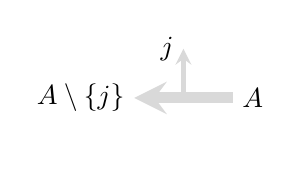
\begin{tikzpicture}
			[scale=1.25,baseline=(current bounding box.center),>=stealth]
				\colorlet{lgray}{white!85!black}
				\draw[lgray,line width=4pt,<-] (0.5,0) -- (1.5,0);
				\draw[lgray,line width=1.5pt,->] (1,0) -- (1,0.5);
				\node[left] at (0.5,0) {$A\setminus\left\{ j \right\}$};
				\node[right] at (1.5,0) {$A$};
				\node[left] at (1,0.5) {$j$};
				\node at (1,-0.5) {};
			\end{tikzpicture}
	\end{equation}
	Here $A\subset\left\{ 1,\ldots,n  \right\}$ is an arbitrary
	subset of colors.
	Denote 
	\begin{equation*}
		\psi(\mu,\nu) \coloneqq \sum_{\textnormal{vertices of the first type in \eqref{eq:psi_factor_two_types_of_vertices}}}
		A_{(j,n]},\qquad 
		A_{(j,n]} \coloneqq \# \left( A\cap \left\{ j+1,\ldots,n  \right\} \right),
	\end{equation*}
	that is, $A_{(j,n]}$
	is the number of arrows of colors
	greater than $j$ which pass over~$j$, when $j$ is inserted from below.

	The conservation of arrows implies that for fixed rows
	$\mu$ and $\nu$ which are interlacing in the sense of \Cref{def:colored_interlacing_triangle},
	there
	is only one configuration of arrows in \eqref{eq:psi_factor_vertex_model}.
\end{definition}

For the colored interlacing triangle in \Cref{fig:small_interlacing_example},
we have $\psi(\lambda^1, \lambda^2) = 2$ and $\psi(\lambda^2, \lambda^3) = 3$.

\medskip\noindent
\textbf{Combinatorial interpretation of $\psi$.}
	The statistic $\psi(\mu, \nu)$ from \Cref{def:psi}
	admits an equivalent description which does not involve a vertex model.
	Consider the transition from level $k$ to level $k+1$.
	For a position $p$ in the linear order \eqref{eq:interlacing_order}
	and a color $c'$, let
	\begin{align*}
		T_{<p}(c') &\coloneqq \#\{\text{level-$(k+1)$ positions of $c'$ that are to the left of $p$}\},\\
		B_{<p}(c') &\coloneqq \#\{\text{level-$k$ positions of $c'$ that are to the left of $p$}\}
	\end{align*}
	denote the number of occurrences of $c'$ in the top and bottom rows,
	respectively, to the left of~$p$.
	Then
	\begin{equation}
		\label{eq:psi_combinatorial}
		\psi(\lambda^{k}, \lambda^{k+1}) =
		\sum_{\text{positions $p$ at level $k$}}
		\ssp\sum_{c' > c(p)}
		\bigl(T_{<p}(c') - B_{<p}(c')\bigr),
	\end{equation}
	where $c(p)$ is the color at position $p$ in level $k$.
	% In words: for each position $p$ in the bottom row (level $k$) carrying color $c$,
	% and for each color $c' > c$, we add the difference between
	% the number of $c'$'s in the top row to the left of $p$
	% and the number of $c'$'s in the bottom row to the left of $p$.

For an example, consider the following 
colored interlacing $4$-triangle of depth~$2$:
\begin{center}
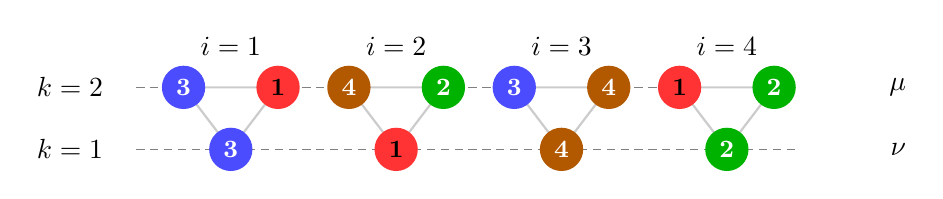
\begin{tikzpicture}
	[scale=0.75,
	 dot1/.style={circle, fill=red!80, minimum size=5.5mm, inner sep=0pt, font=\small\bfseries},
	 dot2/.style={circle, fill=green!70!black, minimum size=5.5mm, inner sep=0pt, font=\small\bfseries, text=white},
	 dot3/.style={circle, fill=blue!70, minimum size=5.5mm, inner sep=0pt, font=\small\bfseries, text=white},
	 dot4/.style={circle, fill=orange!70!black, minimum size=5.5mm, inner sep=0pt, font=\small\bfseries, text=white}]
	\def\h{0.8}
	\def\v{1.05}
	\def\tsep{3.5*\h}
	% Level labels
	\node[left] at (-2.5*\h, 0) {$k=1$};
	\node[left] at (-2.5*\h, \v) {$k=2$};
	\node[left] at (14.5*\h, 0) {$\nu$};
	\node[left] at (14.5*\h, \v) {$\mu$};
	% Dashed level lines
	\draw[gray, densely dashed] (-2*\h,0) -- (3*\tsep+1.5*\h,0);
	\draw[gray, densely dashed] (-2*\h,\v) -- (3*\tsep+1.5*\h,\v);
	% Triangle 1: top (3,1), bot (3)
	\begin{scope}[shift={(0,0)}]
		\draw[gray!40, thick] (-\h,\v) -- (\h,\v) -- (0,0) -- cycle;
		\node[dot3] at (-\h,\v) {3};
		\node[dot1] at (\h,\v) {1};
		\node[dot3] at (0,0) {3};
		\node at (0,\v+0.7) {$i=1$};
	\end{scope}
	% Triangle 2: top (4,2), bot (1)
	\begin{scope}[shift={(\tsep,0)}]
		\draw[gray!40, thick] (-\h,\v) -- (\h,\v) -- (0,0) -- cycle;
		\node[dot4] at (-\h,\v) {4};
		\node[dot2] at (\h,\v) {2};
		\node[dot1] at (0,0) {1};
		\node at (0,\v+0.7) {$i=2$};
	\end{scope}
	% Triangle 3: top (3,4), bot (4)
	\begin{scope}[shift={(2*\tsep,0)}]
		\draw[gray!40, thick] (-\h,\v) -- (\h,\v) -- (0,0) -- cycle;
		\node[dot3] at (-\h,\v) {3};
		\node[dot4] at (\h,\v) {4};
		\node[dot4] at (0,0) {4};
		\node at (0,\v+0.7) {$i=3$};
	\end{scope}
	% Triangle 4: top (1,2), bot (2)
	\begin{scope}[shift={(3*\tsep,0)}]
		\draw[gray!40, thick] (-\h,\v) -- (\h,\v) -- (0,0) -- cycle;
		\node[dot1] at (-\h,\v) {1};
		\node[dot2] at (\h,\v) {2};
		\node[dot2] at (0,0) {2};
		\node at (0,\v+0.7) {$i=4$};
	\end{scope}
\end{tikzpicture}
\end{center}
Let us illustrate teh computation of 
$\psi(\mu,\nu)$ via \eqref{eq:psi_combinatorial}.
For each bottom-row position $p$ with color $c(p)$,
we list the pairs $(T_{<p}(c'),\, B_{<p}(c'))$ for each $c'>c(p)$:
\begin{alignat*}{2}
	c(p)=\textcolor{blue!70}{3}:&\quad c'=4\colon\;(0,0),
	&\qquad& \text{subtotal } 0;\\
	c(p)=\textcolor{red!80}{1}:&\quad c'=2\colon\;(0,0),\  c'=3\colon\;(1,1),\  c'=4\colon\;(1,0),
	&& \text{subtotal } 1;\\
	c(p)=\textcolor{orange!70!black}{4}:&\quad \text{no }c'>4,
	&& \text{subtotal } 0;\\
	c(p)=\textcolor{green!70!black}{2}:&\quad c'=3\colon\;(2,1),\  c'=4\colon\;(2,1),
	&& \text{subtotal } 2.
\end{alignat*}
Hence $\psi(\mu,\nu) = 0+1+0+2 = 3$.

\medskip
Define the \emph{color complement} involution acting on colors by
$\bar{c} = n+1-c$ for each $c \in \{1,\ldots,n\}$,
and extend it to sequences entrywise.
\begin{lemma}[Color complement symmetry]
	\label{lem:color_complement}
	If $\mu = \lambda^k \prec \lambda^{k+1} = \nu$ are interlacing rows in the sense of \Cref{def:colored_interlacing_triangle},
	then $\bar{\mu} \prec \bar{\nu}$, and
	\begin{equation}
		\label{eq:psi_complement}
		\psi(\mu, \nu) + \psi(\bar{\mu}, \bar{\nu}) = k\binom{n}{2}.
	\end{equation}
\end{lemma}
\begin{proof}
	The color complement map preserves the interlacing 
	since it is simply a permutation of colors.
	Now, consider the vertex model in \Cref{def:psi}.
	The statistic $\psi(\mu,\nu)$ counts, for each vertex of the first type in \eqref{eq:psi_factor_two_types_of_vertices}
	with incoming color $j$, the number of colors $j' > j$ that are active (present in $A$).
	Under the bar map, the inequality $j < j'$ becomes $\bar{j} > \bar{j'}$, reversing the color order.
	Thus $\psi(\bar{\mu}, \bar{\nu})$ counts, for each such vertex, the colors $j' > j$ that are \emph{not} active.
	Since there are $k$ vertices of the first type for each color, and each pair $(j, j')$ with $j < j'$
	contributes exactly once per vertex to either $\psi(\mu,\nu)$ or $\psi(\bar{\mu}, \bar{\nu})$,
	the sum equals $k\binom{n}{2}$.
\end{proof}

\subsection{$q$-counting polynomial}
\label{subsec:q_counting_polynomial}

We now define a $q$-deformation of the enumeration of colored interlacing triangles
$T_N(n)$.
\begin{definition}
	\label{def:q_polynomial}
	For a colored interlacing $n$-triangle $\boldsymbol\lambda$ of depth $N$,
	define the \emph{total $\psi$-weight}
\begin{equation*}
		\psi(\boldsymbol\lambda) \coloneqq \sum_{k=1}^{N-1} \psi(\lambda^k, \lambda^{k+1}).
	\end{equation*}
	The \emph{$q$-counting polynomial} is
	\begin{equation*}
		T_N(n;q) \coloneqq \sum_{\boldsymbol\lambda \in \mathcal{T}_N(n)} q^{\psi(\boldsymbol\lambda)}.
	\end{equation*}
	Clearly, at $q=1$, we have $T_N(n;1) = T_N(n) = \#\mathcal{T}_N(n)$.
\end{definition}

\begin{proposition}
	\label{prop:q_polynomial_properties}
	The polynomial $T_N(n;q)$ has the following properties:
	\begin{enumerate}[\rm (i)]
		\item $\deg T_N(n;q) = \binom{n}{2} \cdot \binom{N}{2}$.
		\item $T_N(n;q) = q^{\binom{n}{2}\binom{N}{2}} T_N(n;1/q)$.
		\item $2^{n-1} \mid T_N(n;q)$ as a polynomial
		(that is, all coefficients are divisible by $2^{n-1}$).
	\end{enumerate}
\end{proposition}
\begin{proof}
\begin{enumerate}[\rm (i)]
	\item The maximum value of $\psi(\lambda^k, \lambda^{k+1})$ is $k\binom{n}{2}$
	(achieved when all colors $j' > j$ are active at each level-$k$ vertex of color $j$).
	Summing over $k=1,\ldots,N-1$ gives
	$\sum_{k=1}^{N-1} k\binom{n}{2} = \binom{n}{2}\binom{N}{2}$.

	\item The color complement involution $\bar{\boldsymbol\lambda}$
	is a bijection on $\mathcal{T}_N(n)$, and by \Cref{lem:color_complement},
	we have
	$\psi(\boldsymbol\lambda) + \psi(\bar{\boldsymbol\lambda}) = \binom{n}{2}\binom{N}{2}$.
	This implies the palindromic property of $T_N(n;q)$.

	\item The $n-1$ independent involutions from the proof of \Cref{prop:divisibility_general_depth}
	preserve the $\psi$-statistic, since they do not affect the relative positions of the swapped entries
	within the linear order \eqref{eq:interlacing_order}.
	Thus, all coefficients of $T_N(n;q)$ inherit the divisibility by $2^{n-1}$.\qedhere
\end{enumerate}
\end{proof}

\subsection{$q$-enumeration in the Genocchi case}
\label{subsec:q_genocchi_case}

For depth $N=2$, the polynomial $T_2(n;q)$ is a $q$-analog of the quantity
$T_2(n) = n! \cdot H_n$ from \Cref{thm:Genocchi_counts}.
By \Cref{prop:q_polynomial_properties}, $T_2(n;q)$ is palindromic of degree $\binom{n}{2}$
and divisible by $2^{n-1}$.
The first few values are:
\begin{align*}
T_2(1;q) &= 1, \\
T_2(2;q) &= 2(1+q), \\
T_2(3;q) &= 2^2(1+5q+5q^2+q^3), \\
T_2(4;q) &= 2^3(1+10q+47q^2+52q^3+47q^4+10q^5+q^6), \\
T_2(5;q) &= 2^4(1+15q+132q^2+527q^3+1019q^4+1172q^5+\textnormal{palindrome}).
\end{align*}
See also \Cref{subsec:q_data} for further values.
We notice the linear growth of the coefficient by the first power of $q$:

\begin{proposition}[Linear coefficient]
	\label{prop:linear_coefficient}
	Writing $T_2(n;q) = 2^{n-1}(1 + a_1 q + \cdots)$,
	the linear coefficient satisfies $a_1 = 5(n-2)$ for $n \ge 3$.
\end{proposition}
\begin{proof}
	We need to count the number of 
	depth-2 colored interlacing 
	triangles with $\psi = 1$.
	Let $\lambda^1=\sigma\in S_n$ denote the permutation in the bottom row. 
	We claim that 
	the number of inversions of $\sigma$ must be either $0$ or $1$ to have $\psi = 1$.
	Modulo this claim, let us first finish the computation of $a_1$ for $n\ge3$. 
	We have the following contributions (normalized by $2^{n-1}$, which 
	counts the top-row involutions, see \Cref{cor:Genocchi_divisibility}):
	\begin{enumerate}[$\bullet$]
		\item 
			When $\sigma=\mathrm{id}$ (no inversions), we can achieve $\psi=1$
			by choosing one of the middle $n-2$ bottom positions $c=2,\ldots,n-1$
			to contribute $1$ to $\psi$. This implies that the color crossing this position 
			must be exactly $c+1$, and forces the configuration, up to top-row involutions.
		\item 
			When $\sigma$ is a boundary transposition $(1,2)$ or $(n-1,n)$, there
			are two ways to achieve $\psi=1$ (up to top-row involutions).
			Indeed, for example, the triangle with $\sigma=(2,1,3,4,\ldots,n) $
			may have top row either $(2| 12| 13| 34| 45| \ldots) $, 
			or $(2| 13| 12| 34| 45| \ldots) $,
			where the vertical bars indicate where the bottom row entries are inserted,
			and two entries between bars are unordered (due to top-row involutions).
		\item 
			Finally, when $\sigma$ is one of the $n-2$ internal transpositions
			$(i,i+1)$, $2\le i \le n-2$, one similarly
			sees that there are four ways to achieve $\psi=1$ (up to top-row involutions).
	\end{enumerate}
	The final count is $n-2+4+4(n-3)=5(n-2)$, as claimed.

	\medskip

	It remains to prove the initial claim that
	the number of inversions in $\sigma$ is at most $1$ when $\psi=1$.
	Suppose $\sigma$ has at least two inversions.
	Let the last element in the one-line notation of $\sigma$ 
	which belongs to an inversion be $\gamma$. There are two cases:
	either $\gamma$ is involved in at least two inversions,
	or $\gamma$ is involved in exactly one inversion, and there is another inversion
	in $\sigma$ disjoint from it. 

	In the first case, let $\alpha,\beta>\gamma$ precede $\gamma$ in $\sigma$.
	Suppose that all bottom-row entries to the right of $\gamma$ do not 
	contribute to $\psi$. This means that the top-row entries to the right of $\gamma$'s bottom position
	are uniquely determined (up to top-row involutions). 
	Therefore, both rightmost copies of $\alpha$ and $\beta$ in the top row
	must appear to the left of $\gamma$'s bottom position, yielding $\psi \ge 2$.
	If, on the other hand, we wish to place a top-row $\alpha$ or top-row $\beta$
	to the right of $\gamma$'s bottom position, then there is an entry $\delta>\gamma$ 
	that must go to the left of $\gamma$'s bottom position,
	since we chose $\gamma$ as the last entry participating in an inversion.
	Thus, in the first case, we get $\psi \ge 2$.

	In the second case, let $(\gamma, \delta)$ be the inversion involving $\gamma$
	(so $\delta > \gamma$ precedes $\gamma$ in $\sigma$).
	Since $\gamma$ is the last element participating in an inversion,
	all elements after $\gamma$ in $\sigma$ are in increasing order.
	By interlacing, their top-row copies must fill all positions
	to the right of $\gamma$'s bottom position, otherwise we get at least 
	one contribution to $\psi$ from the right side of $\gamma$.
	But
	this forces both copies of $\delta$ to appear to the left of $\gamma$'s bottom,
	so $\delta$ contributes at least $1$ to $\psi$ at $\gamma$'s position.
	Thus, we see that the inversion $(\gamma, \delta)$ contributes at least $1$ to $\psi$.
	Similarly, the other inversion $(\alpha, \beta)$ also contributes at least $1$ to $\psi$,
	yielding $\psi \ge 2$.
	This completes the proof.
\end{proof}

In \Cref{subsec:conjectures_on_coefficients} below,
we conjecture expressions for the next few coefficients
based on the computed values of $T_2(n;q)$.
\begin{remark}
	\label{rem:psi_vs_inv}
	The proof
	of
	\Cref{prop:linear_coefficient}
	shows that $\psi \ge 2$ whenever $\mathrm{inv}(\sigma) \ge 2$,
	but the inequality $\psi \ge \mathrm{inv}(\sigma)$ does \emph{not} hold in general.
	For example, with $n=3$ and $\sigma = (3,2,1)$, we have $\mathrm{inv}(\sigma) = 3$,
	yet the top row $(3|12|23|1)$ gives $\psi = 2$.
\end{remark}

The polynomials $T_2(n;q)$
are $q$-analogs of $n! \cdot H_n$, and refining them over the bottom row
yields a $q$-analog of the Genocchi median $H_n$ for each permutation $\sigma\in S_n$.
\begin{definition}
	\label{def:H_sigma}
	For any permutation $\sigma \in S_n$, the \emph{$q$-Genocchi median conditioned on $\sigma$} is
	given by
	\begin{equation*}
		H_n^\sigma(q) \coloneqq 
		\sum_{\boldsymbol\lambda \in \mathcal{T}_2(n),\ \lambda^1 = \sigma}
		q^{\psi(\lambda^1, \lambda^2)}.
	\end{equation*}
\end{definition}

For example, for the identity permutation $\mathrm{id} = (1,2,\ldots,n)$, we get:
\begin{align*}
	H_1^{\mathrm{id}}(q) &= 1, \\
	H_2^{\mathrm{id}}(q) &= 2, \\
	H_3^{\mathrm{id}}(q) &= 4(1+q), \\
	H_4^{\mathrm{id}}(q) &= 8(1+  2q + 4q^2), \\
	H_5^{\mathrm{id}}(q) &= 16(1 + 3q + 9q^2 + 16q^3 + 9q^4).
\end{align*}

\begin{proposition}
	\label{prop:H_sigma_properties}
	The polynomials $H_n^\sigma(q)$ have the following properties:
	\begin{enumerate}[\rm (i)]
		\item $2^{n-1} \mid H_n^\sigma(q)$ for all $\sigma \in S_n$.
		\item 
		$H_n^{\bar\sigma}(q) = q^{\binom{n}{2}} H_n^\sigma(1/q)$,
		where $\bar\sigma$ denotes the color complement $\bar\sigma(i) = n+1-\sigma(i)$.
		\item $H_n^{\sigma}(1)=H_n$, the $n$-th Genocchi median, for all $\sigma \in S_n$.
	\end{enumerate}
\end{proposition}
\begin{proof}
\begin{enumerate}[\rm (i)]
	\item The $n-1$ independent involutions from \Cref{prop:divisibility_general_depth}
	preserve both the bottom row and the $\psi$-statistic.

	\item By \Cref{lem:color_complement}, the color complement bijection
	$\boldsymbol\lambda \mapsto \bar{\boldsymbol\lambda}$
	maps triangles with bottom row $\sigma$ to triangles with bottom row $\bar\sigma$,
	and satisfies $\psi(\bar{\boldsymbol\lambda}) = \binom{n}{2} - \psi(\boldsymbol\lambda)$.

	\item When $q=1$, we are just counting the number of colored interlacing triangles
	with a fixed bottom row $\sigma$, and permutations of colors do not affect the interlacing constraints.
	\qedhere
\end{enumerate}
\end{proof}

\begin{remark}
	\label{rem:inverse_not_palindromic}
	The inversion map $\sigma \mapsto \sigma^{-1}$ does \emph{not} induce a relation
	between $H_n^\sigma(q)$ and $H_n^{\sigma^{-1}}(q)$
	similar to the color complement.
	For instance, $\sigma = (1,3,4,2)$ has inverse $\sigma^{-1} = (1,4,2,3)$, and
	$H_4^{(1,3,4,2)}(q) = 8(4q^2 + 3q^3)$ while $H_4^{(1,4,2,3)}(q) = 8(5q^2 + 2q^3)$.
\end{remark}

\begin{remark}
	\label{rem:H_sigma_not_known}
	One can check that the polynomials $H_n^\sigma(q)$ do not coincide with the known $q$-analogs
	of Genocchi medians from \Cref{subsec:known_q_analogs}.
	For instance, the polynomials $H_n^\sigma(q)$ are divisible by $2^{n-1}$,
	while the ones from \Cref{subsec:known_q_analogs} instead contain certain powers of $(1+q)$.
	Even removing these prefactors, the resulting polynomials do not generally match for $n\ge4$.
\end{remark}





%%%%%%%%%%%%%%%%%%%%%%%%%%%%%%%%%%%%%%%%%%%%%%%%%%%%%%%%%%%%%%%%%%%%%%%%%%%%%%%
\section{Computational results and observations}
\label{sec:enumeration}
%%%%%%%%%%%%%%%%%%%%%%%%%%%%%%%%%%%%%%%%%%%%%%%%%%%%%%%%%%%%%%%%%%%%%%%%%%%%%%%

In this section, we present computational data for colored interlacing triangles
beyond the cases covered by \Cref{thm:Genocchi_counts} and \cite{gaetz2023bijection}.

\subsection{Computation of new values of $T_N(n)$}
\label{subsec:computational_approach}

We computed new values of $T_N(n)$ using a level-by-level dynamic programming approach
with GPU acceleration.
The code related to this subsection is available at
the following GitHub repository:
\begin{equation}
	\label{eq:colored_interlacing_triangles_enumeration_github}
	\text{\url{https://github.com/lenis2000/colored_interlacing_triangles_enumeration/}}
\end{equation}

We enumerate interlacing colored triangles
$\boldsymbol\lambda = (\lambda^1 \prec \lambda^2 \prec \cdots \prec \lambda^N)$
by computing, for each level $k = 1, \ldots, N-1$,
the number of ways to extend each configuration $\lambda^k$ to a compatible $\lambda^{k+1}$.
We enumerate only configurations in $\mathring{\mathcal{T}}_N(n)$,
that is, those with $\lambda^1=(1,2,\ldots,n)$.
Moreover, 
in generating candidates for $\lambda^{k+1}$, 
we exploit the $2^{n-1}$-symmetry from
\Cref{prop:divisibility_general_depth},
and also restrict the search to sequences $\lambda^{k+1}$
which start with $1$ and end with $n$. 
To obtain $T_N(n)$, we multiply the final count by $n!\ssp 2^{n-1}$.

\begin{table}[h]
	\centering
	\small
\begin{tabular}{|c|c|c|c|c|c|c|c|}
	\hline
	$T_N(n)\rule{0pt}{13pt}$       & $n=2$                 & $n=3$   & $n=4$      & $n=5$       & $n=6$     & \ldots & $n$           \\[2pt] \hline
        $N=1$  & 2                     & 6       & 24         & 120         & 720       & \ldots & $n!$          \\ \hline
				$N=2$  & 4                     & 48      & 1,344      & 72,960      & 6,796,800 & \ldots & $n!\cdot H_n$ \\ \hline
				$N=3$  & 8                     & 528     & 191,232    & 257,794,560 & 1,012,737,392,640         & \ldots & \textbf{?}             \\ \hline
				$N=4$  & 16                    & 8,160   & 72,099,840 & ?           & ?         & \ldots & \textbf{?}             \\ \hline
				$N=5$  & 32                    & 179,520 & 73,410,306,048          & ?           & ?         & \ldots & \textbf{?}             \\ \hline
				$N=6$  & 64                    & 5,666,304 & ?          & ?           & ?         & \ldots & \textbf{?}             \\ \hline
				\ldots & \ldots                & \ldots  & \ldots     & \ldots      & \ldots    & \ldots & \ldots        \\ \hline
				$N$    & $2^N$\rule{0pt}{12pt} & $\tfrac14\mathfrak{g}_N^{\Delta}(4)$   & \textbf{?}          & \textbf{?}           & \textbf{?}         & \ldots &               \\[3pt] \hline
    \end{tabular}
		\caption{Known and unknown values of $T_N(n)$, the number of colored interlacing $n$-triangles with $N$ levels.
		Bold-faced question marks indicate unknown series of values.
		The columns $n=2$ and $n=3$ are \cite{ABW2023coloured_LLT}
		and \cite{gaetz2023bijection}, respectively.
		The row $N=2$ is our \Cref{thm:Genocchi_counts}.}
	\label{tab:known_counts_of_colored_interlacing_triangles}
\end{table}

We implemented the interlacing checks on Apple Metal GPU, achieving throughput
of about $1$~to~$2$ billion checked pairs per second on an M2 Pro chip.
For large state spaces exceeding available memory (e.g., $T_5(4)$), we process
target states in batches of $50$ million with intermediate results accumulated.
The results of the computations are summarized in \Cref{tab:known_counts_of_colored_interlacing_triangles}.
All of the counts took less than a second to compute,
except for $T_3(6)$, which took about $14$ minutes,
and $T_5(4)$, which took about $9$ hours.

Beyond the values reported in \Cref{tab:known_counts_of_colored_interlacing_triangles} and the known cases $N\le 2$ or $n\le 3$, 
the number of configurations to be checked
at the final level grows extremely rapidly, and the 
required computation time stretches to multiple days or weeks.

The elements in \Cref{tab:known_counts_of_colored_interlacing_triangles}
contain large prime factors. For instance, 
$T_5(4)$ is divisible by 331,897, and $T_3(6)$ is divisible by 457,871,
and both of these divisors are primes.
This indicates that a simple product formula
for the $T_N(n)$'s is highly unlikely.
On the other hand, the $2$-adic valuations 
(that is, the highest powers of $2$ dividing the numbers)
of the normalized counts
$T_N(n)/n!$ may
exhibit certain patterns, see \Cref{tab:2_adic_valuations}.

\begin{table}[htpb]
	\centering
	\begin{tabular}{|c|c|c|c|c|c|}
		\hline
		 & $n=2$ & $n=3$ & $n=4$ & $n=5$ & $n=6$ \\
		\hline
		$N=1$ & 0 & 0 & 0 & 0 & 0 \\
		\hline
		$N=2$ & 1 & 3 & 3 & 5 & 5 \\
		\hline
		$N=3$ & 2 & 3 & 5 & 6 & 10 \\
		\hline
		$N=4$ & 3 & 4 & 8 & ? & ? \\
		\hline
		$N=5$ & 4 & 5 & 10 & ? & ? \\
		\hline
	\end{tabular}
	\caption{$2$-adic valuations of the normalized counts $T_N(n)/n!$.}
	\label{tab:2_adic_valuations}
\end{table}

\subsection{Computation of $q$-polynomials for two levels}
\label{subsec:q_data}

We computed the $q$-counting polynomials $T_2(n;q)$
defined in \Cref{sec:q_enumeration}
by 
finding the statistic $\psi$ for all
colored interlacing triangles of depth $N=2$.
The code and data of the statistic $\psi$ are
available at the following GitHub repository:
\begin{equation}
\label{eq:colored_interlacing_triangles_q_enumeration_github}
\text{\url{https://github.com/lenis2000/colored_interlacing_triangles_q_enumeration}}
\end{equation}

For $N=2$, a colored interlacing $n$-triangle consists of
a permutation $\lambda^1 \in S_n$ (level~$1$) and
a sequence $\lambda^2$ of length $2n$ where each color appears exactly twice (level~$2$).
The interlacing condition requires that for each color $c$, its position in
$\lambda^1$ lies strictly between its two positions in $\lambda^2$.

The algorithm explores the same symmetries as in \Cref{subsec:computational_approach} to 
reduce the search space.
For each ``canonical'' triangle from $\mathring{\mathcal{T}}_2(n)$
(with identity permutation at level~$1$),
we compute the $\psi$-statistic for all $n!$ color permutations in the whole triangle.
Namely,
for each valid interlacing triangle $(\lambda^1, \lambda^2)$,
we compute $\psi(\lambda^1, \lambda^2)$ using bitmask operations:
we process positions right-to-left, maintaining a bitmask of ``active'' colors
(those that have entered from the right but not yet exited upward).
The contribution to the $q$-power is computed via hardware-accelerated population count
(\texttt{popcount}) instructions.
The available data on GitHub also accounts for the distribution of $q$-statistics over all $n!$ permutations
for each canonical triangle.

The implementation uses \texttt{C++} template metaprogramming to specialize the inner loop for each $n$,
enabling complete loop unrolling and instruction-level parallelism (processing 4 permutations
simultaneously). Combined with OpenMP parallelization, we achieve the following benchmarks
on an Apple M2 Pro (6 performance cores):
\begin{center}
{\renewcommand{\arraystretch}{1.15}%
\setlength{\tabcolsep}{8pt}%
\begin{tabular}{c|r|r}
\hline
$n$ & \multicolumn{1}{c|}{Canonical triangles} & \multicolumn{1}{c}{Time} \\ \hline
6 & 295 & $< 1$ second \\
7 & 3,098 & $< 1$ second \\
8 & 42,271 & $\approx 28$ seconds \\
9 & 726,734 & $\approx 1$ hour \\ \hline
\end{tabular}}
\end{center}

Writing $T_2(n;q) = 2^{n-1} P_n(q)$, the polynomials $P_n(q)$ are
of degree $\binom{n}{2}$ and are 
palindromic (indicated by the symbol $\circlearrowleft$ below).
Here are their explicit forms for $n$ up to $9$:
\begin{align*}
P_1(q) &= 1, \\
P_2(q) &= 1+q, \\
P_3(q) &= 1+5q+5q^2+q^3, \\
P_4(q) &= 1+10q+47q^2+52q^3+47q^4+10q^5+q^6, \\
P_5(q) &= 1+15q+132q^2+527q^3+1019q^4+1172q^5+\circlearrowleft
, \\
P_6(q) &= 1+20q+245q^2+1825q^3+7295q^4+19534q^5+34465q^6 
+42815q^7+\circlearrowleft, \\
P_7(q) &= 1+25q+383q^2+3977q^3+26645q^4+115165q^5+365346q^6 \\
&\quad +878276q^7+1563964q^8+2226948q^9+2626230q^{10}+\circlearrowleft, \\
P_8(q) &= 1+30q+546q^2+7018q^3+64622q^4+411692q^5+1914780q^6 \\
&\quad +6889907q^7+19865655q^8+46208719q^9+88274748q^{10} \\
&\quad +141139717q^{11}+193232778q^{12}+231337829q^{13}+245670636q^{14} +\circlearrowleft,\\
P_9(q) &=
1 + 35q + 734q^2 + 11064q^3 + 125319q^4 + 1059757q^5 + 6649287q^6 + 32573212q^7\\
&\quad+ 129428316q^8 + 424672873q^9 + 1174423848q^{10} + 2770263242q^{11} + 5640036376q^{12} 
\\&\quad
+ 9998171117q^{13} + 15583534941q^{14} + 21645762974q^{15} + 27163602028q^{16}
\\&\quad
+ 31055190622q^{17} + 32466222428q^{18} + \circlearrowleft.
\end{align*}

\begin{conjecture}
	\label{conj:log_concavity}
	The coefficients of each polynomial $P_n(q)$ are log-concave:
	if $P_n(q) = \sum_{k} a_k(n) q^k$, then 
	we have $a_k(n)^2 \ge a_{k-1}(n) a_{k+1}(n)$ for all $n,k$.
	We have verified this for $n \le 9$.
\end{conjecture}

\subsection{Coefficients of $P_n(q)$}
\label{subsec:conjectures_on_coefficients}

We implemented a different strategy to access low-degree
coefficients of $P_n(q)$ 
beyond $n=9$,
where the full polynomial computation becomes too slow.
The code for this approach is available at the repository
\eqref{eq:colored_interlacing_triangles_q_enumeration_github}.

Rather than generating all Dumont derangements
for a given $n$ (corresponding to interlacing triangles of depth $2$
with identity permutation at the bottom row) and then computing the $\psi$-statistics
for all $n!$ permutations of colors,
we \emph{invert the loops}: the outer loop iterates over all $n!$ bottom row permutations $\lambda^1$,
while the inner loop generates Dumont derangements on-the-fly via backtracking.
The key observation is that the $\psi$-statistic accumulates during the
backtracking process. When computing only coefficients by $q^k$ for
$k<K_{\max}$ (with $K_{\max}$ small),
we prune any branch where the partial $\psi$-value reaches $K_{\max}$.
This pruning eliminates a large portion of the Dumont search space.

A further optimization exploits the relationship between the inversion number
of the bottom row permutation $\lambda^1$ and the $\psi$-statistic.
Empirically, permutations with large inversion numbers tend to produce only
high $\psi$-values across all Dumont derangements.
By restricting to bottom row permutations with $\operatorname{inv}(\lambda^1) \leq I_{\max}$
for a suitable threshold $I_{\max}$,
we reduce the outer loop dramatically while still capturing all contributions
to low-degree coefficients.
Combined, these optimizations make it feasible to compute low-degree coefficients
up to $n = 15$. We obtain the following
initial pieces of further polynomials $P_n(q)$:
\begin{align*}
	P_{10}(q) &= 1 + 40q + 947q^2 + 16240q^3 + 214297q^4 + 2207081q^5 \ldots,
	\\
	P_{11}(q) &= 1+45q + 1185q^2 + 22671q^3 + 338129q^4 +4033256 q^5\ldots,
	\\
	P_{12}(q) &= 1 + 50q + 1448q^2 + 30482q^3 + 504040q^4 +6762968 q^5 \ldots,
	\\
	P_{13}(q) &= 1 + 55q + 1736q^2 + 39798q^3 + 719880q^4 +10663371q^5 \ldots,
	\\
	P_{14}(q) &= 1 + 60q + 2049q^2 + 50744q^3 + 994124q^4 +16045700 q^5 \ldots,
	\\
	P_{15}(q) &= 1 + 65q + 2387q^2 + 63445q^3 + 1335872q^4 + 23268315 q^5 \ldots.
\end{align*}

Based on this data, we conjecture the following polynomial behavior of all the remaining coefficients
of $P_n(q)$, with concrete polynomials for the next four (recall that the linear coefficient is $a_1(n)=5(n-2)$, see \Cref{prop:linear_coefficient}):
\begin{conjecture}
\label{conj:coeff_polynomials}
For each fixed $k \geq 0$, and all $n\ge n_0(k)$, the coefficient $a_k(n)$
of $q^k$ in $P_n(q)$ is 
a polynomial in $n$ of degree $k$. Specifically, we conjecture the following 
polynomials for the next four coefficients:
\begin{equation}
\label{eq:conj_coeff_polynomials}
\begin{split}
	 a_2(n)&=\frac{25n^2 - 49n - 116}{2},\qquad n \geq 5,\\
	 a_3(n)&=\frac{125n^3 + 15n^2 - 3104n + 1980}{6},\qquad  n \geq 7,\\
	 a_4(n)&=\frac{625 n^4 + 2650 n^3 - 36877 n^2 - 31390 n + 244728}{24},\qquad  n \geq 9,\\
	a_5(n)&=\frac{3125 n^5 + 32500 n^4 - 290925 n^3 - 1585240 n^2 + 7120060 n + 5588400}{120},\qquad  n \geq 11.
\end{split}
\end{equation}
\end{conjecture}
\begin{conjecture}[Leading coefficient]
\label{conj:leading_coefficient}
As polynomials in $n$, the expressions
$k!\ssp a_k(n)$
have integer coefficients for all $k \geq 0$,
and their leading coefficient is $5^k$.
\end{conjecture}
\begin{remark}
	\label{rmk:log_concavity}
	The polynomials \eqref{eq:conj_coeff_polynomials} (together with $a_1(n)=5n-10$) satisfy log-concavity 
	$a_k(n)^2 \ge a_{k-1}(n) a_{k+1}(n)$ for $k=2,3,4$ and all $n>0$. This 
	supports our \Cref{conj:log_concavity}.
\end{remark}

\begin{proof}[Evidence for \Cref{conj:leading_coefficient}]
Let us briefly explain why one expects
\[
a_k(n)=\frac{5^k}{k!}\,n^k+O(n^{k-1}),\qquad n\to\infty.
\]
In the proof of \Cref{prop:linear_coefficient}, for each \emph{internal} interface between the $i$-th and $(i+1)$-st bottom positions ($i\in\{2,\ldots,n-2\}$), there are \emph{five} canonical local modifications (modulo the $2^{n-1}$ involutions) which create exactly one unit of $\psi$ while keeping the rest of the triangle as forced as possible: one coming from $\sigma=\mathrm{id}$ and four coming from $\sigma$ having a single adjacent transposition $(i,i+1)$. Each such modification is confined to a bounded window around that interface and contributes exactly $1$ to~$\psi$.

Fix $k$ and choose $k$ internal interfaces $i_1<\cdots<i_k$ with $i_{r+1}\ge i_r+2$, so the corresponding windows are disjoint. Starting from the canonical $\psi=0$ configuration, we may independently insert at each $i_r$ one of the five local defects; disjointness prevents interactions, so the resulting triangle has $\psi=k$. Hence
\[
a_k(n)\ \ge\ 5^k\cdot M_{n,k},
\]
where $M_{n,k}$ is the number of $k$-subsets of $\{1,\ldots,n-1\}$ with no adjacent elements (equivalently, $k$-matchings in a path of length $n-1$). Thus,
\[
M_{n,k}=\binom{n-k}{k}=\frac{1}{k!}n^k+O(n^{k-1}),
\qquad\text{and so}\qquad
a_k(n)\ \ge\ \frac{5^k}{k!}n^k+O(n^{k-1}).
\]

Conversely, for fixed $k$ the condition $\psi=k$ is expected (and consistent with all computed data) to force the triangle to differ from the canonical $\psi=0$ configuration only at $O(k)$ such local interfaces. Any overlaps of defect windows, boundary effects, or other interactions reduce the number of free choices by at least one, contributing only $O(n^{k-1})$ possibilities. Thus the top-degree term should come precisely from choosing $k$ independent internal defect locations (a $k$-matching) and, at each, one of the $5$ defect types, giving the desired leading term.
\end{proof}

\subsection{Linear cumulant phenomenon}
\label{subsec:linear_cumulant_phenomenon}

If we apply the classical ``moment-cumulant'' transformation 
(corresponding to taking the logarithm of the exponential generating function)
to the sequence of
the normalized coefficients
$m_k(n)\coloneqq k!\ssp a_k(n)$ coming from 
\eqref{eq:conj_coeff_polynomials}, then we obtain the following linear functions of $n$:
\begin{equation*}
\begin{split}
	m_1&=5n-10,\\
	m_2-m_1^2&=51n-216,\\
	m_3-3m_2m_1+2m_1^3
	&=166n-3500,\\
	m_4
	-4m_3m_1-3m_2^2+12m_2m_1^2-6m_1^4
	&=-28854n+84360,\\
	m_5
	-5m_4m_1-10m_3m_2+
	20m_3m_1^2+30m_2^2m_1-60m_2m_1^3+24m_1^5
	&=
	- 1258080 n
	+10684800 .
\end{split}
\end{equation*}
\begin{conjecture}
	This pattern of linear cumulants continues for all $k\ge1$.
\end{conjecture}
	
The linear cumulant phenomenon aligns with the local independence
picture discussed after 
\Cref{conj:coeff_polynomials,conj:leading_coefficient}:
if the $\psi$-statistic arises from choosing independent local defects
at disjoint interfaces, then the distribuion of $\psi$
should be approximately a sum of independent random variables, 
one per interface.
For such sums, cumulants grow linearly in the number of summands.

\subsection{Moment sequences}
\label{subsec:moment_sequences}

By agreement,
let us add the initial value $T_2(0;q)=1$.
Let us consider the question 
whether the sequence $T_2(n;q)=2^{n-1}P_n(q)$, $n\ge0$,
is a Stieltjes moment sequence in $n$ for each fixed $q\in[0,1]$,
that is, there exists a nonnegative Borel measure $\mu_q$ on $[0,+\infty)$
such that
\begin{equation*}
	T_2(n;q) \;=\; \int_{0}^{+\infty} x^n \, d\mu_q(x), \qquad n=0,1,2,\ldots.
\end{equation*}
We know that this is the case for $q=0$ and $q=1$:
\begin{equation*}
	T_2(n;0) =\begin{cases}
		1, & n=0; \\
		2^{n-1}, & n\ge1,
	\end{cases}
	\qquad 
	T_2(n;1) = n! \cdot H_n.
\end{equation*}
Indeed, for $q=0$, we have $\mu_0=\frac{1}{2}\delta_0+\frac{1}{2}\delta_2$,
and for $q=1$, the sequences $\{n!\}$ and $\{H_n\}$ are both Stieltjes moment
sequences, so their product is also a Stieltjes moment sequence.

For other values of $q\in(0,1)$, we employ 
the classical test based on two Hankel determinants, 
$\det[ T_2(i+j-2;q) ]_{i,j=1}^k$ and
$\det[ T_2(i+j-1;q) ]_{i,j=1}^k$,
for $k$ up to $5$.
We find that both determinants may be negative for sufficiently
small $q>0$, for instance:
\begin{equation*}
	\det[ T_2(i+j-2;q) ]_{i,j=1}^5<0,\qquad 0<q<c_1, \qquad 
	c_1\approx 0.08462\ldots,
\end{equation*}
and 
\begin{equation*}
	\det[ T_2(i+j-1;q) ]_{i,j=1}^3<0,\qquad 0<q<c_2, \qquad
	c_2\approx 0.04641\ldots.
\end{equation*}
The values $c_1$ and $c_2$ are the smallest positive roots
of the respective determinants viewed as polynomials in $q$.
Thus, for 
sufficiently small $q>0$,
the sequence $\{T_2(n;q)\}_{n\ge0}$ is not a Stieltjes moment sequence
in~$n$.
Since the property holds at the endpoints $q=0$ and $q=1$,
the moment sequence property undergoes a transition
at $q=0^+$, ruling out a uniform representation of $T_2(n;q)$
as moments of a family of nonnegative Borel measures varying in $q$ over $[0,1]$.




%%%%%%%%%%%%%%%%%%%%%%%%%%%%%%%%%%%%%%%%%%%%%%%%%%%%%%%%%%%%%%%%%%%%%%%%%%%%%%%
\section{Sampling depth-$2$ colored interlacing triangles}
\label{sec:sampling}
%%%%%%%%%%%%%%%%%%%%%%%%%%%%%%%%%%%%%%%%%%%%%%%%%%%%%%%%%%%%%%%%%%%%%%%%%%%%%%%

Here, we describe a simple Markov chain
which preserves the 
$q$-weighted distribution on depth-$2$ colored interlacing triangles.
That is, each triangle $\boldsymbol\lambda\in\mathcal{T}_2(n)$
is sampled with probability proportional to $q^{\psi(\boldsymbol\lambda)}$.
The code is available at the GitHub repository
\begin{equation}
\label{eq:colored_interlacing_triangles_sampling_github}
\text{\url{https://github.com/lenis2000/colored_interlacing_triangles_q_sampling}}
\end{equation}

Define a 
Markov chain 
on the state space $\mathcal{T}_2(n)$
that
uses two types of local moves.

\begin{definition}[Level-$2$ swap]
\label{def:level2_swap}
Given a position $p \in \{1, \ldots, 2n-1\}$,
the \emph{level-$2$ swap at position $p$} exchanges $\lambda^2_p$ and $\lambda^2_{p+1}$.
The move is \emph{valid} if the resulting configuration still satisfies the interlacing constraint.
\end{definition}

\begin{definition}[Level-$1$ swap with reconciliation]
\label{def:level1_swap}
Given a position $i \in \{1, \ldots, n-1\}$,
let $a = \lambda^1_i$ and $b = \lambda^1_{i+1}$.
The \emph{level-$1$ swap at position $i$} exchanges $a$ and $b$ in $\lambda^1$,
then applies a deterministic \emph{reconciliation} to $\lambda^2$ to restore interlacing.

Let the \emph{between region} consist of positions $\lambda^2_{2i-1}$ and $\lambda^2_{2i}$
(the level-$2$ entries that lie between the $i$-th and $(i+1)$-st positions in the linear order \eqref{eq:interlacing_order}).
The reconciliation proceeds as follows:
\begin{enumerate}[\rm (i)]
\item If neither $a$ nor $b$ appears in the between region, no change to $\lambda^2$ is needed.
\item If only $a$ appears in the between region, replace it with $b$,
then a copy of $b$ to the right of the between region, and replace it with $a$.
\item If only $b$ appears in the between region, then act symmetrically to (ii):
replace $b$ with $a$ in the between region,
then replace a copy of $a$ to the left of the between region with $b$.
\item If both $a$ and $b$ appear in the between region, find $a$ to the left of the between region
and $b$ to the right, and swap them.
\end{enumerate}
This move is always valid: one readily sees that interlacing is preserved.
\end{definition}

\begin{proposition}[Connectedness of the state space]
\label{prop:connected_state_space}
The two types of swaps from \Cref{def:level1_swap,def:level2_swap}
connect all states in $\mathcal{T}_2(n)$.
\end{proposition}
\begin{proof}
We show that any triangle can be transformed to the identity one with
$\lambda^1 = (1, 2, \ldots, n)$ and $\lambda^2 = (1, 1, 2, 2, \ldots, n, n)$.
First, level-1 swaps can sort $\lambda^1$ to the identity permutation. 
The reconciliation ensures that $\lambda^2$ is adjusted to maintain interlacing.

Second, once $\lambda^1 = (1, 2, \ldots, n)$, the level-$2$ swaps can rearrange $\lambda^2$
within the constraints imposed by interlacing.
Indeed, one copy of $1$ in the second level is fixed at position $1$.
Let us move the other copy of $1$ to position $2$ using level-$2$ swaps
which move $1$ leftward. The only obstruction to the leftward movement of $1$
is a configuration of the form
$(\ldots b a|a|1c\ldots)$, which 
prevents swapping $1$ and $a$ on the second level. However, since $a\ne b$, 
we can first swap $a$ and $b$ on the second level, and then swap $1$ and $b$, 
resulting in the configuration $(\ldots 1a|a|bc\ldots)$.
This allows to proceed with moving $1$ leftward.
After the other copy of $1$ is at position $2$, we can remove the leftmost triangle consising 
of all $1$'s, and repeat the same procedure for $2,3,\ldots,n$.
\end{proof}

We can thus apply the \emph{Metropolis--Hastings} (also called the \emph{Markov Chain Monte Carlo}) \emph{algorithm} with our swaps. In
detail,
at each step, uniformly choose one of the $3n-2$
possible swap positions at both levels, attempt the corresponding move (in particular, check the validity
of the level-2 swap), and accept or reject according to the
Metropolis--Hastings rule with acceptance probability
\begin{equation*}
	\alpha(\boldsymbol\lambda \to \boldsymbol\lambda')
	= \min\bigl(1, q^{\psi(\boldsymbol\lambda') - \psi(\boldsymbol\lambda)}\bigr).
\end{equation*}
It is well-known
\cite{LevinPeres2017}
that this procedure defines a Markov chain
with stationary distribution proportional to $q^{\psi(\boldsymbol\lambda)}$.

\medskip
The results of sampling are illustrated in
\Cref{fig:sampled_triangles,fig:sampling_heatmaps,fig:psi_histogram}.
The effect of the $q$-weighting is visible both in the sampled triangles
and in the heatmaps. The latter resemble the permuton limit of the Mallows
measure on permutations 
\cite{Starr2009}.
\Cref{fig:psi_histogram} shows the empirical distribution of the $\psi$-statistic;
it looks approximately Gaussian.

\begin{figure}[htpb]
\centering
% q=0.2, psi=55
\resizebox{\textwidth}{!}{%
\begin{tikzpicture}[y=4.5cm]
\foreach \c/\lpos/\ltpos/\rtpos in {%
1/1/1/3, 2/3/4/9, 3/2/2/6, 4/5/5/12, 5/7/8/15, 6/8/10/16, 7/9/14/20, 8/4/7/19,%
9/10/13/23, 10/6/11/17, 11/14/21/32, 12/11/18/25, 13/13/24/31, 14/15/28/34, 15/12/22/35, 16/19/27/39,%
17/18/33/36, 18/17/30/37, 19/20/26/40, 20/16/29/42, 21/21/41/44, 22/25/38/57, 23/26/47/52, 24/24/46/48,%
25/22/43/50, 26/23/45/53, 27/27/49/55, 28/28/54/56, 29/30/59/63, 30/33/62/69, 31/29/51/60, 32/32/61/64,%
33/34/65/77, 34/36/66/72, 35/37/68/75, 36/35/67/70, 37/31/58/73, 38/40/76/81, 39/39/74/79, 40/38/71/89,%
41/42/82/85, 42/43/80/90, 43/41/78/84, 44/44/83/88, 45/45/86/93, 46/46/91/92, 47/48/94/96, 48/47/87/97,%
49/49/95/98, 50/50/99/100%
}{%
\pgfmathsetmacro{\hue}{\c/50}%
\definecolor{col}{hsb}{\hue,0.8,0.8}%
\draw[col, line width=2pt] ({\lpos-1},0) -- ({\ltpos*0.5-0.5},1);%
\draw[col, line width=2pt] ({\lpos-1},0) -- ({\rtpos*0.5-0.5},1);%
\fill[col] ({\lpos-1},0) circle (7pt);%
\fill[col] ({\ltpos*0.5-0.5},1) circle (7pt);%
\fill[col] ({\rtpos*0.5-0.5},1) circle (7pt);%
}
\end{tikzpicture}}

\vspace{1em}

% q=0.98, psi=541
\resizebox{\textwidth}{!}{%
\begin{tikzpicture}[y=4.5cm]
\foreach \c/\lpos/\ltpos/\rtpos in {%
1/16/27/49, 2/3/3/37, 3/10/15/53, 4/35/31/82, 5/25/17/73, 6/5/9/67, 7/29/36/64, 8/33/51/81,%
9/11/7/40, 10/44/41/97, 11/15/28/33, 12/39/30/80, 13/1/1/44, 14/13/16/60, 15/45/19/91, 16/38/63/96,%
17/19/23/65, 18/34/50/92, 19/48/54/99, 20/2/2/76, 21/50/57/100, 22/4/4/26, 23/14/5/39, 24/47/34/94,%
25/12/18/43, 26/31/14/69, 27/6/11/71, 28/28/21/77, 29/24/20/74, 30/17/12/42, 31/42/70/84, 32/37/52/89,%
33/20/38/56, 34/23/13/66, 35/46/62/95, 36/9/8/25, 37/26/45/72, 38/40/46/83, 39/41/24/87, 40/49/93/98,%
41/36/58/75, 42/7/6/90, 43/8/10/79, 44/18/32/47, 45/43/61/86, 46/21/22/59, 47/32/48/85, 48/22/35/78,%
49/27/29/68, 50/30/55/88%
}{%
\pgfmathsetmacro{\hue}{\c/50}%
\definecolor{col}{hsb}{\hue,0.8,0.8}%
\draw[col, line width=2pt] ({\lpos-1},0) -- ({\ltpos*0.5-0.5},1);%
\draw[col, line width=2pt] ({\lpos-1},0) -- ({\rtpos*0.5-0.5},1);%
\fill[col] ({\lpos-1},0) circle (7pt);%
\fill[col] ({\ltpos*0.5-0.5},1) circle (7pt);%
\fill[col] ({\rtpos*0.5-0.5},1) circle (7pt);%
}
\end{tikzpicture}}
\caption{Sampled depth-$2$ colored interlacing triangles with $n=50$ colors,
	ordered as a rainbow from color $1$ (red) to color $50$ (violet).
	The two triangles were obtained after MCMC runs of 
	$10^7$ steps each.
	Top: $q=0.2$ (here the $\psi$-statistic is $55$).
	Bottom: $q=0.98$ (here $\psi=541$).
	Lines connect each color's occurrences across levels, and indicate the interlacing properties.}
\label{fig:sampled_triangles}
\end{figure}

\begin{figure}[htpb]
	\centering
	\includegraphics[height=0.24\textheight]{heatmap_q02_level1.png}
	\hfill
	\includegraphics[height=0.24\textheight]{heatmap_q02_level2.png}

	\vspace{0.5em}

	\includegraphics[height=0.24\textheight]{heatmap_q09_level1.png}
	\hfill
	\includegraphics[height=0.24\textheight]{heatmap_q09_level2.png}
	\caption{Position frequency heatmaps from
	$10^5$ samples collected after $10^6$ ``burn-in'' steps, with $10^4$ steps between samples
	(so, a total of $10^9$ MCMC steps), where $n=25$.
	Left column: Level~$1$ ($n \times n$). Right column: Level~$2$ ($n \times 2n$).
	Top row: $q=0.2$. Bottom row: $q=0.9$.}
	\label{fig:sampling_heatmaps}
\end{figure}

\begin{figure}[htpb]
	\centering
	\includegraphics[width=0.7\textwidth]{psi_histogram_q09.png}
	\caption{Empirical distribution of $\psi$ with $n=25$, $q=0.9$, from the same samples
	as in \Cref{fig:sampling_heatmaps}.}
	\label{fig:psi_histogram}
\end{figure}






%%%%%%%%%%%%%%%%%%%%%%%%%%%%%%%%%%%%%%%%%%%%%%%%%%%%%%%%%%%%%%%%%%%%%%%%%%%%%%%

\bibliographystyle{alpha}
\bibliography{bib}


\medskip

\textsc{N. Blitvic, Queen Mary University of London, School of Mathematical Sciences, London, UK}

E-mail: \texttt{n.blitvic@qmul.ac.uk}

\medskip

\textsc{L. Petrov, University of Virginia, Department of Mathematics, Char\-lottes\-ville, VA, USA}

E-mail: \texttt{lenia.petrov@gmail.com}


\end{document}
